\section{Graph theory}
Because of the network structure of FPGAs, it is easy to model them as graphs. If we model FPGA components as combinations of vertices and connections, we have a complete representation of an FPGA suitable for graph algorithms.

A graph representation of the physical structure of FPGAs allows us to scan through the structure of the concrete FPGA graph and look for structures that resemble the graph of the virtual FPGA. Let us, for example, assume that the structure of the concrete FPGA graphs contains a complete embedding of the virtual FPGA graph. Then, by disabling each component outside of this embedding and by copying configurations from components in the virtual FPGA model to their respective components in the concrete FPGA graph model, we would have an emulation function. Obtaining this function could entail changing some bits if, for example, the second output of a virtual LUT is mapped to the first output of the concrete LUT and vice versa.\footnote{While virtual components may also be emulated by structures of multiple concrete components connected in specific ways, we deem finding such emulations out of scope for this research.}

The graph-theoretic name for finding these embeddings is subgraph isomorphism. It is an NP-complete problem\cite{cook} with many algorithms explored. The problem with using an approach of subgraph isomorphism is, however, that many possible emulations cannot be found. For example, a concrete FPGA may have much more configurable routing switches than a virtual FPGA. A subgraph isomorphism algorithm would in this case not find an emulation, even though one is technically possible by configuring some routing switches to function as wires.

A variant of subgraph isomorphism is (vertex disjoint) subgraph homeomorphism. In this problem, intermediate vertices are allowed in the embedding on the target-graph side. This means that the embedding consists of a vertex-to-vertex mapping and an edge-to-path mapping.

This is the essence of our research: finding some subset of the concrete FPGA (using graphs) that is topologically the same way as the virtual FPGA and has the appropriate components that can emulate virtual components one-to-one.

\begin{defn}[graph]
A graph is a tuple $(V, E, L)$ where $V$ is a set of vertices, $E$ is a multiset of directed edges such that each edge $e \in E \to e \in (V \times V)$ and $L: (V \to \mathbb{P}(\lambda))$ is a multilabelling function where $\lambda$ is a finite alphabet.
\label{def:graph}
\end{defn}


\begin{defn}[(vertex disjoint) subgraph homeomorphism]
Let $P$ the set of all loopless paths in $G_T$, let $\mathit{first}(p)$ be the first vertex of a path $p$, let $\mathit{last}(p)$ be the last vertex of a path $p$ and let $\mathit{intermediate}(p)$ be all other vertices of a path $p$. Then, a subgraph homeomorphism from graph $S$ to graph $T$ is a tuple $(\mathit{vmap}, \mathit{emap})$ where $\mathit{vmap}\subseteq (V_S \mapsto V_T)$ and $\mathit{emap} \subseteq (E_S \mapsto P)$ are both injective functions such that:

\begin{tabular}{rlr}
 1. & $\forall s \in V_S . L_S(s)\subseteq L_T(\mathit{vmap}(s))$&\\
 
 &i.e. vertices are mapped to vertices that have at least the same label set.&\\
 
 2. & $\forall (s_1, s_2) \in E_S .\mathit{first}(\mathit{emap}(s_1, s_2))=\mathit{vmap}(s_1) \land \mathit{last}(\mathit{emap}(s_1, s_2))=\mathit{vmap}(s_2)$&\\
 &i.e. each edge in $G_1$ is mapped to a path in $G_2$.&\\
 
 3. & $\forall p \in \mathit{values}(\mathit{emap}) . \forall x \in \mathit{intermediate}(p) . $\\
 &$\quad \not \exists p' \in (\mathit{values}(\mathit{emap}) \setminus \{p\}) . x \in \mathit{intermediate}(p')$&\\
    &i.e. these paths are internally vertex disjoint.&\\
\end{tabular}

This tuple is also the certificate for the decision problem of subgraph homeomorphism, which returns whether a tuple like this exists. A popular different way to define the decision problem is whether the target graph contains a subgraph which can be obtained by repeatedly intersecting the source graph's edges with vertices.

\label{def:pathsubgraphisomorphism}
\end{defn}


\begin{figure}
\centering
\parbox{1.2in}{

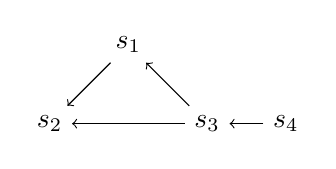
\begin{tikzpicture}
\node at (0,1) (a) {$s_1$};
\node at (1,0) (c)  {$s_3$};
\node at (-1,0) (b)  {$s_2$};
\node at (2,0) (d)  {$s_4$};

\draw[->] (a)->(b);
\draw[->] (c)->(a);
\draw[->] (c)->(b);
\draw[->] (d)->(c);
\end{tikzpicture}
}
\qquad\qquad
\begin{minipage}{1.2in}%

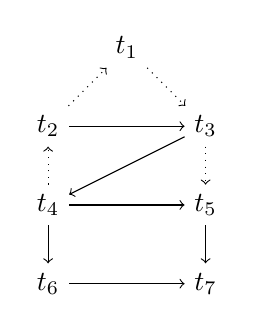
\begin{tikzpicture}
\node at (0,3) (alpha) {$t_1$};
\node at (-1,2) (beta)  {$t_2$};
\node at (1,2) (gamma)  {$t_3$};
\node at (-1,1) (delta)  {$t_4$};
\node at (1,1) (epsilon)  {$t_5$};
\node at (-1,0) (zeta)  {$t_6$};
\node at (1,0) (eta)  {$t_7$};

\draw[dotted, ->] (beta)->(alpha);
\draw[dotted, ->] (alpha)->(gamma);
\draw[->] (beta)->(gamma);
\draw[dotted, ->] (delta)->(beta);
\draw[->] (delta)->(epsilon);
\draw[->] (gamma)->(delta);
\draw[->] (epsilon)->(eta);
\draw[dotted, ->] (gamma)->(epsilon);
\draw[->] (zeta)->(eta);
\draw[->] (delta)->(zeta);

\end{tikzpicture}
\end{minipage}
\caption{Two graphs $G_1$ and $G_2$. $G_1$ is (node disjoint) subgraph homeomorphic to $G_2$ with the mapping $\{(s_1, t_5), (s_2, t_7), (s_3, t_4), (s_4, t_2), (s_1 \to s_2, t_5 \to t_7), (s_3 \to s_1, t_4 \to t_5), (s_3 \to s_2, t_4 \to t_6 \to t_7), (s_4 \to s_3, t_2 \to t_3 \to t_4)\}$. Other homeomorphisms exist as well.}
\end{figure}

Suppose we have graphs $G_{virtual}$ and $G_{concrete}$. In that case, wherever a subgraph homeomorphism from $G_{virtual}$ to $G_{concrete}$ exists, it describes a mapping where the logic of the virtual FPGA may be performed on the concrete FPGA in an emulation\footnote{If no such relation exists, it does not mean a function $f$ as specified in Section \ref{sec:Objectives} does not exist. Emulation could still be obtained by emulation of components by (multiple) components of possibly different types or by emulation of routing switches by sets of connected routing switches.}\footnote{This does not hold if some vertices in $G_{concrete}$ that are part of the mapping are unconfigurably connected and their mapped equivalents in $G_{virtual}$ are not. We account for this in our algorithm with the methods described in Section \ref{sec:unintendedcurrent}.}. The vertex-to-vertex mapping $\mathit{vmap}$ describes how to obtain configurations for the concrete FPGA and the edge-to-path mapping $\mathit{emap}$ describes how vertices in the concrete FPGA are connected via paths of intermediate components configured as wires.


The similarity between \textit{subgraph isomorphism} and \textit{subgraph homeomorphism} allows us to take inspiration from existing subgraph isomorphism algorithms and use similar methods to solve subgraph homeomorphism and therewith the FPGA emulation problem.

